\section{问题二：基于离散制氨调节的运行优化}

\subsection{问题分析与求解思路}

问题二背景设定园区制氨产能增至72吨/日，电氢氨装置仅有全额开机和停机两种运行方式，无需考虑低产量要求时两种产氢设备的产能分配问题。需要确定在满足不同产量水平（72、63、54、45、36吨/日）下成本最低的生产时段安排。产能扩容后对应设备参数线性提升：ALKEL功率上限20 MW、PEMEL功率上限20 MW、合成氨装置功率上限1.5 MW，电氢氨总额定功率$P_{H2NH3}^{max} = 41.5$ MW。每种产量对应的开机时数为$k = Q_{NH3} / 3.0$小时。
\begin{figure}[H]
\centering
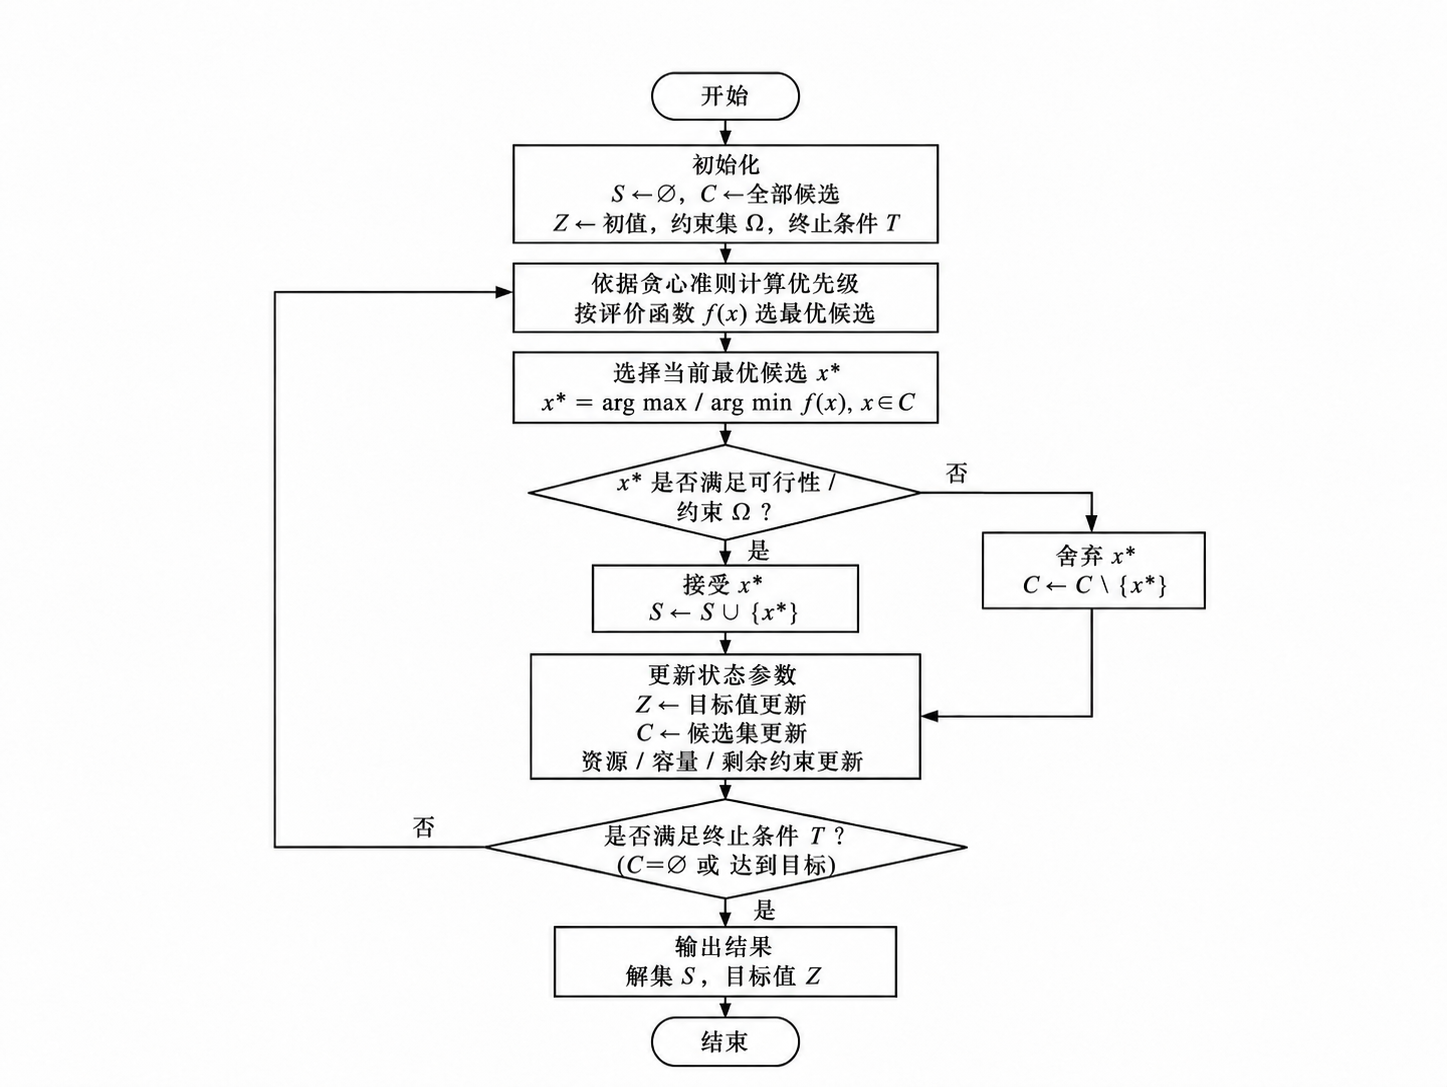
\includegraphics[width=0.8\textwidth,height=0.3\textheight,keepaspectratio]{ChatGPT Image 2026年5月24日 19_04_03.png}
\caption{贪心算法原理图}
\label{fig:placeholder}
\end{figure}

本文采用贪心算法（原理图如图\ref{fig:placeholder}所示）对建立模型求解获得全局最优解\cite{ref2}。该问题的核心是在24个时段中选择$k$个时段开机运行，使得日运行总成本最小。由于每个时段的开机边际成本可独立计算且时段间无耦合约束（无最小开停机时间等约束），在本问题中采用贪心策略的优势有：可将目标函数分解为各时段独立贡献之和，通过选取边际成本最低的$k$个时段即等价于求解原问题的最优解，计算复杂度低。

\subsection{数学模型建立}

\subsubsection{决策变量}

引入二进制决策变量$u(t) \in \{0, 1\}$，$t = 1, 2, \ldots, 24$，其中$u(t) = 1$表示时段$t$电氢氨装置全额开机运行，$u(t) = 0$表示停机。

\subsubsection{约束条件}

\textbf{产量约束：}要求总开机时数等于目标产量对应的小时数：
\begin{equation}\label{eq:q2_production}
\sum_{t=1}^{24} u(t) = k = \frac{Q_{NH3}}{r_{NH3}} = \frac{Q_{NH3}}{3.0}
\end{equation}

\textbf{功率平衡约束：}
\begin{equation}
P_{buy}(t) - P_{sell}(t) = P_{load}(t) + u(t) \cdot P_{H2NH3}^{max} - P_{wind}(t) - P_{pv}(t)
\end{equation}

\textbf{购售电非负约束：}
\begin{equation}
\begin{cases}
    P_{buy}(t) \geq 0\\
    P_{sell}(t) \geq 0
\end{cases}
\end{equation}

\subsubsection{目标函数}

最小化日运行总成本：
\begin{equation}\label{eq:q2_obj}
\min \{C_{day}\} = C_{RE} + \sum_{t=1}^{24} \lambda_{buy}(t) \cdot P_{buy}(t) \cdot \Delta t + \sum_{t=1}^{24} u(t) \cdot C_{OM,h} - \lambda_{sell} \cdot E_{sell}
\end{equation}

其中每小时运维成本为：
\begin{equation}
C_{OM,h} = c_{ALKEL} \cdot P_{ALKEL}^{max} + c_{PEMEL} \cdot P_{PEMEL}^{max} + c_{NH3} \cdot P_{NH3}^{max} = 5003 \text{ 元/h}
\end{equation}

\subsubsection{贪心算法求解}

由于各时段间无耦合约束，目标函数可分解为各时段的独立边际成本之和。定义时段$t$的开机边际成本为：
\begin{equation}\label{eq:greedy_marginal}
\Delta C(t) = C_{on}(t) - C_{off}(t)
\end{equation}
 
\quad \quad \quad \quad \quad $\mathbf{C_{on}(t)}$：时段$t$开机时的运行成本（含购电/售电和运维）
    
\quad \quad \quad \quad \quad $\mathbf{C_{off}(t)}$：停机成本。


具体地：

当净负荷$P_{net}(t) = P_{load}(t) + P_{H2NH3}^{max} - P_{wind}(t) - P_{pv}(t) > 0$时：
\begin{equation}
C_{on}(t) = \lambda_{buy}(t) \cdot P_{net}(t) \cdot 1000 + C_{OM,h}
\end{equation}

当$P_{net}(t) \leq 0$时（有余电可售）：
\begin{equation}
C_{on}(t) = -\lambda_{sell} \cdot |P_{net}(t)| \cdot 1000 + C_{OM,h}
\end{equation}

贪心策略为：按$\Delta C(t)$从小到大排序，选取前$k$个时段开机。该策略的时间复杂度为$O(24\log 24)$，相对于其它优化算法，如指数级运算复杂度的MILP，本算法求得全局最优解的速度优势明显。

\subsection{问题二(1)：典型场景各产量最优方案}

在典型风光场景下，对五种产量水平分别应用贪心算法，得到最优生产时段安排及对应的运行指标，结果如表\ref{tab:q2_typical}所示。

\begin{table}[H]
\centering
\caption{典型场景下各产量水平最优方案（贪心算法）}\label{tab:q2_typical}
\begin{tabular}{ccccccc}
\toprule
日产量(吨) & 开机时数 & 吨氨成本(元/吨) & 设备利用率 &$R_{self}$ & $R_{green}$ & $R_{grid}$ \\
\midrule
72 & 24h & 6219.14 & 100\% & 86.5\% & 53.3\% & 6.7\% \\
63 & 21h & 5328.06 & 87.5\% & 84.3\% & 59.7\% & 7.8\% \\
54 & 18h & 4591.27 & 75\% & 80.2\% & 67.3\% & 9.9\% \\
45 & 15h & 3944.54 & 62.5\% & 51.0\% & 66.7\% & 24.5\% \\
36 & 12h & 3191.67 & 50\% & 10.5\% & 59.7\% & 44.8\% \\
\bottomrule
\end{tabular}
\end{table}

从\textbf{吨氨成本}角度看，产量越低则吨氨成本越低，36吨/日对应最低吨氨成本3191.67元/吨。这是因为低产量方案可以将开机时段集中在风光出力充足且电价低的时段，大幅减少购电需求。然而从\textbf{绿电指标}角度看，低产量方案的指标严重不达标：36吨/日方案的$R_{self}=10.5\%$远低于60\%要求，$R_{grid}=44.8\%$远超20\%上限，原因在于开机时段过短导致大量余电上网。

\begin{figure}[H]
\centering
\includegraphics[width=0.5\textwidth,height=0.2\textheight,keepaspectratio]{../figures/fig_q2_cost_vs_production.pdf}
\caption{不同日产氨量下的吨氨成本变化趋势}\label{fig:q2_cost_vs_production}
\end{figure}

在典型日风光场景下，吨氨成本随产量增加呈单调递增趋势（图\ref{fig:q2_cost_vs_production}），从36吨/日的3191.67元/吨上升至72吨/日的6219.14元/吨。这一趋势的经济学解释是：产量增加意味着更多时段需要开机，被迫在风光出力不足的夜间高电价时段运行，购电成本大幅增加。

\begin{figure}[H]
\centering
\includegraphics[width=0.65\textwidth,height=0.25\textheight,keepaspectratio]{../figures/fig_q2_schedule_gantt.pdf}
\caption{各产量水平下最优开停机时段安排}\label{fig:q2_schedule_gantt}
\end{figure}

最优开机时段安排呈现明显规律（图\ref{fig:q2_schedule_gantt}）：低产量方案优先选择白天光伏高峰时段开机，随着产量增加逐步向夜间扩展。绿电指标全满足的最优产量为54吨/日（$C_{ton}=4591.27$元/吨），此时$R_{self}=80.2\%>60\%$、$R_{green}=67.3\%>30\%$、$R_{grid}=9.9\%<20\%$，三项指标均满足政策要求。该产量对应18小时开机，设备利用率为75\%。

\subsection{问题二(2)：24种场景全年统计分析}

将6种风电出力水平与4种光伏出力水平组合，形成24种风光出力场景。对每种场景分别应用贪心算法求解五种产量水平的最优时段安排，选取吨氨成本最低的方案作为该场景的最优运行策略。得到对应情境最优决策下园区的制氨生产时段安排、相应的绿电直连指标、吨氨成本、园区日购电、售电等指标
\\\textbf{制氨生产时段安排}

对$24 \times 5$种场景分别代入本题模型进行贪心算法求解，得到120组最优生产时段安排，模型运行得到数据大致呈现如下特征：\textbf{从产量上看}，由于日氨产量约束，在最高日氨产量的条件下，所有场景均需要全天24小时开机；随着产量要求下降，风光出力的差异开始体现在时段安排差异上，在大部分风光场景中时段安排与典型日无差别，但在弱光伏场景由于白天发电量不足，在综合电价后，将开机时段转移到低电价时段（详细时段安排见附件）。
\\\textbf{吨氨成本}

\begin{figure}[H]
\centering
\includegraphics[width=0.8\textwidth,height=0.35\textheight,keepaspectratio]{../figures/fig_q2_scenarios_heatmap.pdf}
\caption{24种风光场景$\times$5种产量水平吨氨成本热力图}\label{fig:q2_scenarios_heatmap}
\end{figure}

24种场景与五种产量水平组合下的吨氨成本分布呈现显著差异（图\ref{fig:q2_scenarios_heatmap}）。热力图横轴为日产氨量（72至36吨/日），纵轴为24种风光出力场景。可以观察到：高风电、高光伏场景（如W1P1）在各产量水平下的吨氨成本均较低；低产量方案在所有场景下成本均低于高产量方案，但绿电指标不达标。风电出力水平对成本的影响大于光伏，主要原因在于夜间时段光伏发电功率为0，仅靠风力发电支持，购电需求受风电影响大，直接影响成本。
\\\textbf{绿电直连指标}

按照每种场景代表15天的假设，全年360天的绿电直连指标满足情况统计如表\ref{tab:q2_annual}所示。

\begin{table}[H]
\centering
\caption{问题二全年绿电直连指标统计}\label{tab:q2_annual}
\begin{tabular}{lcc}
\toprule
类别 & 场景数 & 对应天数 \\
\midrule
全满足（三项均达标） & 0种 & 0天 \\
部分满足（1--2项达标） & 21种 & 315天 \\
全不满足（三项均不达标） & 3种 & 45天 \\
\bottomrule
\end{tabular}
\end{table}

在离散调节模式下，全年没有任何场景能够同时满足三项绿电直连指标要求。这一结果说明，仅靠开停机调度无法有效解决风光出力与用电负荷的时序匹配问题，需要引入更灵活的功率调节手段,即后续模型调整方向。
\\\textbf{全年吨氨成本及总成本}

\begin{figure}[H]
\centering
\includegraphics[width=0.6\textwidth,height=0.2\textheight,keepaspectratio]{fig_q2_annual_cost (1).pdf}
\caption{全年吨氨成本分布曲线}\label{fig:q2_annual_cost}
\end{figure}

基于模型给出数据将24种风光场景依次排序后得到全年吨氨成本分布曲线（图\ref{fig:q2_annual_cost}）。其中在最低产量要求下，24种场景的吨氨成本从1370.40元/吨到7125.16元/吨不等，全年平均吨氨成本为4494元/吨，全年总产量为9720吨。成本分布呈现较大离散度，反映了风光出力随机性对园区经济性的显著影响。
